\section{Конструкторская часть}
\newsection{Конструкторская часть}
В конструкторской части приводится структура разрабатываемого
программного обеспечения. Описывается назначение каждого модуля и
основные алгоритмы функционирования сети. На основе вышеизложенного,
представим высокоуровневый протокол взаимодействия участников сети и
обмен протоколом.

\subsection{Структура программного обеспечения}
Приложение состоит из процесса клиента, процесса сервера и
пользовательского приложения. При этом процессы клиент и сервер является
демонами, то есть не могут непосредственно взаимодействовать с
пользователем. Приведем небольшую схему структуры программного
обеспечения ниже на рисунке \ref{pic_1}.
\begin{figure}[!hbt]
    \centering
    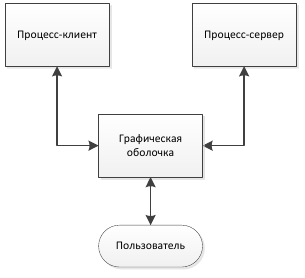
\includegraphics{pic_1}
    \caption{Структура программного обеспечения}\label{pic_1}
\end{figure}

На рисунке выше видно, что пользователь может взаимодействовать только с
графической оболочкой, графическая оболочка в свою очередь
взаимодействует с сервером и клиентом.

\subsection{Алгоритм работы клиента}
Приведем описание работы клиента. Описываемый здесь алгоритм клиента
не показывает взаимодействие клиента с остальными компонентами сети,
взаимодействие показано ниже. Приведем словесное описание того как
функционирует процесс, затем приведем схему алгоритма.
\newpar
Клиент запускается в момент запуска приложения, является процессом-демоном.
Процесс-клиент (или просто клиент) выполняет следующие
функции:
\begin{enumerate}
    \item при появлении в сети нового участника, клиент заносит его в список
        пассивных подключений;\label{enum:client}
    \item вызывает диспетчера (во время получения файла);\label{enum:disp}
    \item обрабатывает запросы, которые могли прийти от сервера или от
        GUI.\label{enum:gui}
\end{enumerate}

Ниже подробнее опишем данные функции.
\newpar
Рассмотрим последовательность действий выполняемых, когда клиент
получает сообщение от сервера или GUI (пункт \ref{enum:gui}). При получении
сообщения от GUI клиент вызывает обработчик запросов GUI и выполняет
некоторые действия, в числе которых может быть и завершение работы
клиента. Сообщение, получаемое клиентом от сервера, содержит кусок файла
и информацию, которая описывает каким образом обрабатывать данный
кусок файла. Данное сообщение передается callback-функции, которая
десериализует полученное сообщение и проверяет его на наличие ошибок,
если они присутствуют, то возвращается ошибка. Иначе происходит
идентификация пакета (определяется, какой уникальной передачи относится
получаемый пакет), если, идентификация неуспешна, то возвращается
ошибка, иначе вызывается функция, которая обрабатывает полученный кусок
файла. Данная функция выполняет следующие действия:
\begin{enumerate}
    \item если идентификатор файла отрицательное число, то возвращает
        управление и выводит сообщение об ошибке;
    \item иначе, копирует содержимое файла в список полученных кусков;
    \item если число подряд идущих кусков (то есть идентификаторы кусков
        расположены в списке в порядке возрастания) достигает
        определенной величины, то данные сбрасываются на жесткий диск.
\end{enumerate}

При получении некоторого куска файла он не сбрасывается на диск сразу, так
как в данном случае происходило бы частое обращение к жесткому диску
(запись данных на жесткий диск занимает относительно много времени, так
как связана с механическими действиями), что сказалось бы на общей
производительности.
\begin{figure}[!hbt]
    \centering
    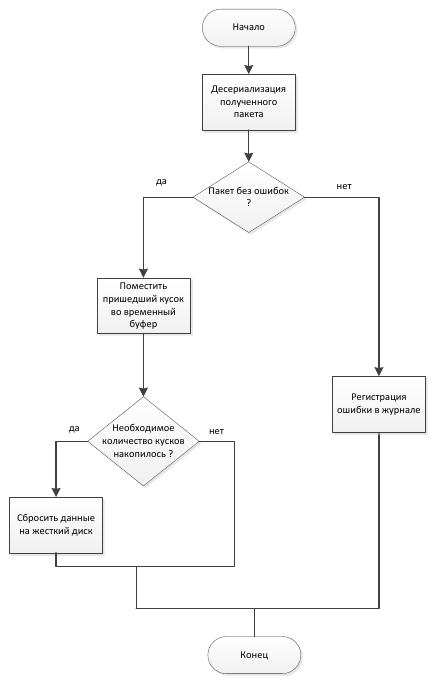
\includegraphics{pic_2_2}
    \caption{Блок-схема алгоритма процедуры обработки получаемых пакетов}\label{pic_2}
\end{figure}
\newpar
Для решения данной проблемы куски заносятся во
временный буфер, когда в буфере накапливается определенная
последовательность кусков, которые следуют друг за другом, то содержимое
сбрасывается на жесткий диск. На рисунке \ref{pic_2}, приведена блок-схема (далее
схема) алгоритма работы процедуры <<Обработчик данных>>, которая
обрабатывает получаемые пакеты.
\newpar
Другой функций клиента является добавление новых участников (пункт \ref{enum:client}).
\newpar
Если в сети появился новый участник, то вызывается функция, которая
добавляет этого участника в список пассивных подключений. Ниже, на
рисунке \ref{pic_3}, видно в какой момент происходит добавление нового участника
сети.

\begin{figure}[!hbtp]
    \centering
    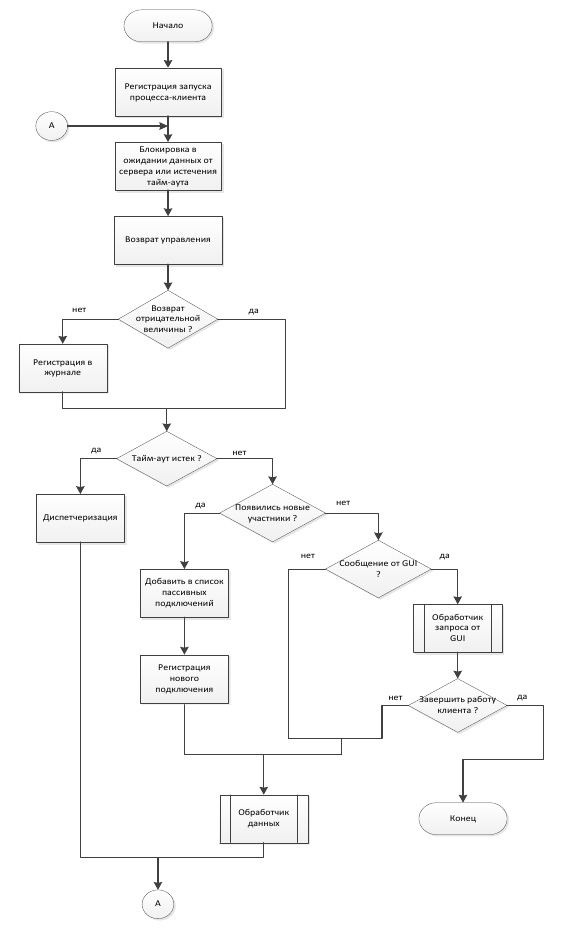
\includegraphics[scale=0.9]{pic_3}
    \caption{Блок-схема алгоритма работы клиента}\label{pic_3}
\end{figure}

\newpage
\subsection{Алгоритм работы сервера}
Приведем описание алгоритма работы сервера, который включает рассылку
широковещательных сообщений и передачу файлов при запросе от клиента.
Как и выше опишем алгоритм работы сервера словесно, а далее приведем
схему.
\newpar
Сервер, который, как и клиент является процессом-демоном, запускается в
момент запуска приложения. При этом процесс-сервер при запуске запускает
поток, тем самым работа сервера разделяется на следующие две задачи,
которые выполняются независимо друг от друга:
\begin{enumerate}
    \item поток, порожденный основным процессом, производит рассылку
        широковещательных сообщений всем участникам сети;
    \item основной процесс ожидает получения запроса на передачу
        некоторого куска.
\end{enumerate}

Поток, отвечающий за рассылку широковещательных сообщений,
порождается сразу при запуске основного процесса-сервера. После удачного
запуска он производит широковещательную рассылку сообщений участникам
сети.
\newpar
Основной процесс после удачного запуска ожидает запроса на передачу
некоторого файла, который посылается некоторым участником сети.
Ожидание происходит путем блокирования процесса на системном вызове
select. Данный системный вызов используется для организации
мультиплексирования ввода-вывода, который описывается далее. Когда
сервер получает сообщение от клиента, которое также является
последовательностью байтов и содержит информацию о куске файла который
необходимо передать клиенту, он (сервер) проверяет наличие файла на хосте.
В случае успеха он считывает кусок файла и передает его клиенту, иначе
передает клиенту сообщение об ошибке, то есть информирует клиента о том,
что запрашиваемый файл отсутствует.
\newpar
Ниже, на рисунке \ref{pic_4} приведем общую схему работы основного процесса-сервера,
схема работы потока приводиться не будет, так как алгоритм
достаточно простой. Также как и в процессе-клиенте, используется системная
функция select, которая может вернуть отрицательное значение. Данный факт
будет регистрироваться в журнале, однако процесс-сервер не будет прерывать
свою работу, так как данная ошибка не является критической.

\begin{figure}[!p]
    \centering
    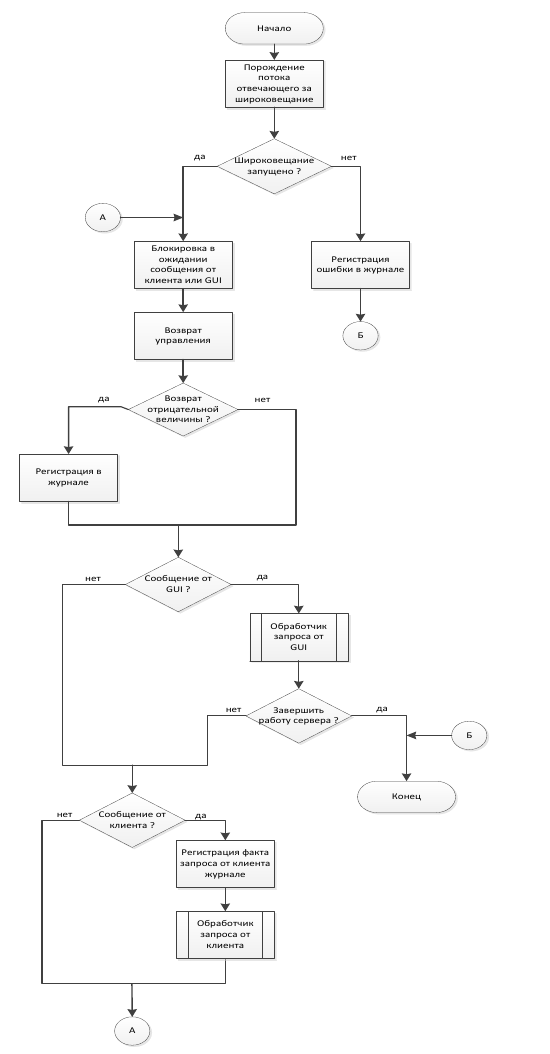
\includegraphics[scale=0.88]{pic_4}
    \caption{Блок-схема алгоритма работы сервера}\label{pic_4}
\end{figure}

\newpar
Процедура, которая обрабатывает запросы пришедшие серверу, будет описана
ниже на рисунке \ref{pic_5}, также будет приведена схема этой процедуры.

\begin{figure}[!p]
    \centering
    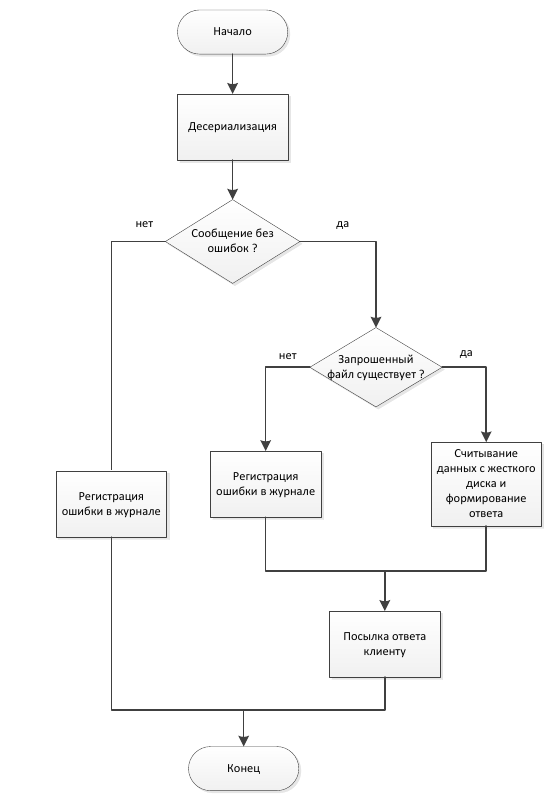
\includegraphics[width=\textwidth]{pic_5}
    \caption{Блок-схема алгоритма процедуры обработки запроса сервером}\label{pic_5}
\end{figure}

\newpar
На схеме, приведенной на рисунке \ref{pic_4}, происходит вызов процедуры <<Обработчик
запроса от клиента>>, данная процедура обрабатывает запросы, пришедшие от
других участников сети. Опишем алгоритм работы данной процедуры.
\newpar
Процедура <<Обработчик запроса от GUI>> принимает и обрабатывает
сообщение от GUI, которое может быть только сообщением о завершении
работы сервера.
\newpar
При вызове процедуры обработки запроса от клиента ей передается
сообщение, а именно протокол в виде последовательности байт. Далее
происходит десериализация, если она успешна, то процедура продолжает
работу, иначе выход с ошибкой. Ошибка может произойти, если полученное
сообщение имеет неверный формат, иначе происходит обработка запроса и
формирование ответа. При формировании ответа сервер проверяет наличие
запрашиваемого файла и в случае успеха пересылает клиенту тот кусок
файла, который запросил клиент, иначе передается сообщение об ошибке.
\newpar
На рисунке \ref{pic_5}, приведена схема работы процедуры обработки запроса.

\subsection{Взаимодействие с пользовательским приложением}
В основном, взаимодействие сервера и клиента с графической оболочкой
сводится к обмену некоторой информацией о состоянии передачи или число
участников в сети.
\newpar
Перед началом передачи файла клиент должен получить информацию о том
файле, который необходимо запросить у серверов. Данная информация
передается клиенту пользовательским приложением
(графической оболочкой). Для этого использовался текстовый формат передачи данных
JSON.

\subsection{Взаимодействие клиента и сервера}
Выше были описаны алгоритмы работы клиента и сервера, а также
получение запроса на передачу файла. Теперь опишем алгоритм
взаимодействия клиента и сервера. Подразумевается, что клиент и сервер
находятся на разных хостах.
\newpar
Когда необходимо получить некоторый файл клиент получает информацию о
нем из пользовательского приложения (GUI). Получив информацию о файле,
который необходимо получить, клиент заносит всех из списка пассивных
подключений в список активных подключений, далее проходит по списку
активных подключений, и посылает каждому запрос на передачу куска файла,
который необходимо получить. Сервер, получив запрос от клиента на
передачу куска файла, проверяет наличие файла на хосте и в случае успеха
пересылает клиенту запрашиваемый кусок файла. Иначе посылает
сообщение, в котором указано, что на данном сервере нет запрашиваемого
файла. Клиент начинает получать различные куски файлов и действует
согласно выше описанному алгоритму. Если какой-либо сервер присылает
сообщение об отсутствие файла, клиент удаляет из списка активных
соединений, то есть в последствие не запрашивает данный файл у этого
сервера. Во время передачи файла может возникнуть ситуация, когда
некоторый сервер не отвечает определенное время либо завершил свою
работу, не переслав необходимые данные. В таком случае, кусок файла
возвращается в список запрашиваемых кусков и будет запрошен повторно.

\subsection{Алгоритм планирования}
Опишем алгоритм планирования запросов для получения кусков.
\newpar
Данный алгоритм реализуется клиентом. Размер куска файла определяется
как некоторая константа. Планирование происходит по следующим правилам:
\begin{enumerate}
    \item клиент логически разбивает файл на куски, каждый из которых
        имеет одинаковый размер;
    \item каждый кусок нумеруется в порядке возрастания;
    \item следующим будет запрошен минимальный кусок из списка
        отвергнутых кусков, если он не пуст, иначе кусок с минимальным
        порядковым номером, который еще не был запрошен;
    \item если некоторый кусок, не может быть получен от сервера, то он
        помещается в список отвергнутых кусков для того, чтобы быть
        запрошенным как можно раньше.
\end{enumerate}

\subsection{Алгоритм функционирования приложения}
Ниже, на рисунках \ref{pic_6}, \ref{pic_7} и \ref{pic_8} приведем блок-схему функционирования приложения,
при этом в ней не будем приводить алгоритмы функционирования клиента и
сервера, так как они приведены выше. То есть, данная схема отображает
только логику работы приложения.

\begin{figure}[!p]
    \centering
    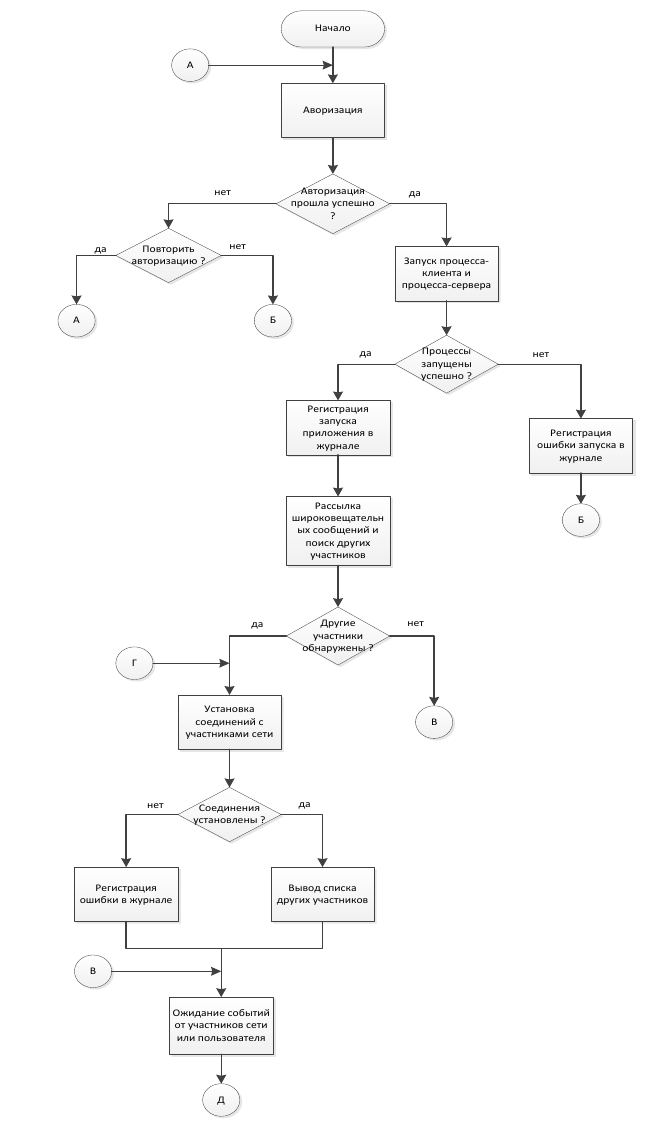
\includegraphics[scale=0.8]{pic_6}
    \caption{Блок-схема алгоритма функционирования приложения}\label{pic_6}
\end{figure}

\begin{figure}[!p]
    \centering
    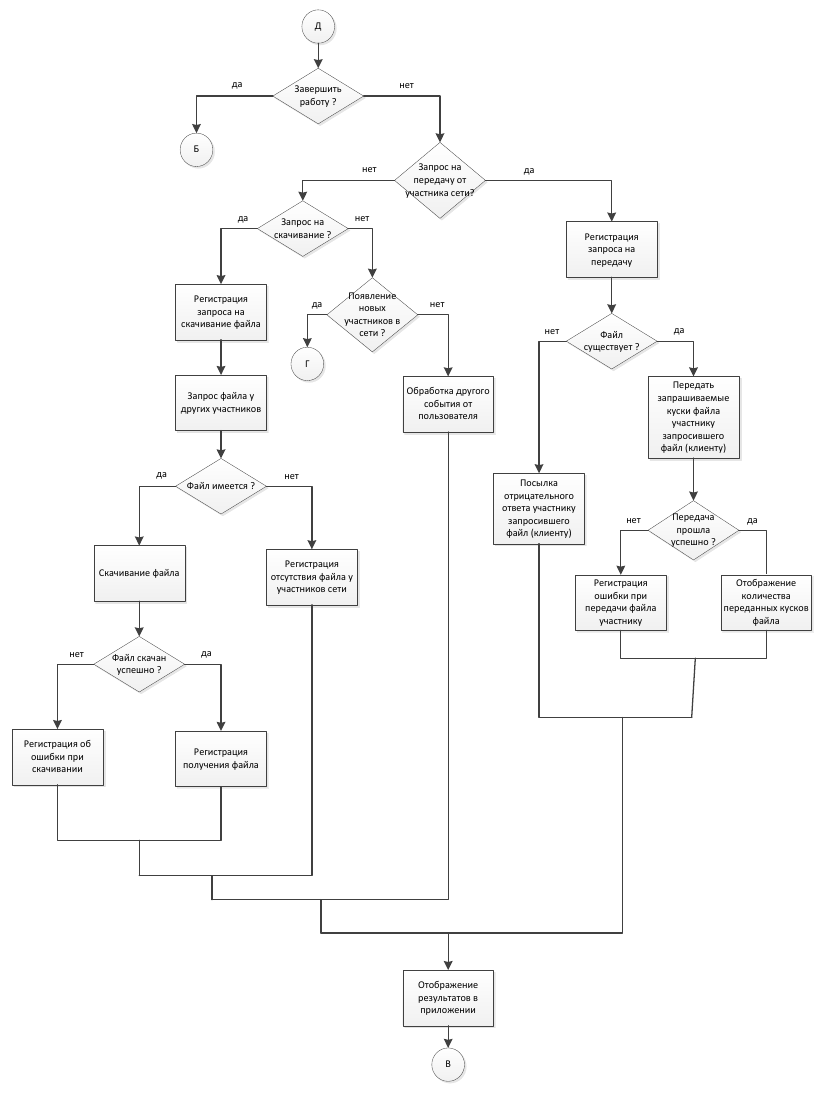
\includegraphics[scale=0.8]{pic_7}
    \caption{Блок-схема алгоритма функционирования приложения (продолжение)}\label{pic_7}
\end{figure}

\newpage
\begin{figure}[t!]
    \centering
    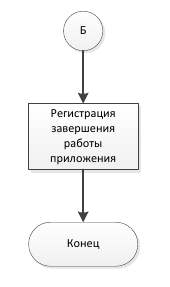
\includegraphics[scale=0.8]{pic_8}
    \caption{Блок-схема алгоритма функционирования приложения (продолжение)}\label{pic_8}
\end{figure}

\subsection{Схема взаимодействия участников сети}
Приведем схему взаимодействия в сети, на которой отобразим то, как
происходит взаимодействие между участниками сети.
\newpar
Под участником сети здесь будем понимать приложение, которое было
запущено на хосте. Как описывалось выше, каждое приложение состоит из
процесса-клиента, процесса-сервера и пользовательского приложения,
которое предоставляет графический интерфейс пользователю.
\newpar
Ниже, на рисунке \ref{pic_9}, приведена схема взаимодействия нескольких участников сети. На
этой схеме, процесс-сервер и процесс-клиент показаны в блоках <<Сервер i>> и
<<Клиент i>> соответственно. Блок пользовательского приложения имеет
соответствующее название <<Пользовательское приложение i>>, где i~-- номер
участника сети. Стрелками будем указывать направления обмена
сообщениями. Номера стрелок соответствуют следующим сообщениям:
\begin{enumerate}
    \item посылка широковещательного сообщения всем участникам сети,
        широковещание производится сервером, передача куска файла запрошенного
        клиентом или посылка сообщения о том, что у данного сервера отсутствует
        запрашиваемый файл.
    \item сообщения от других участников сети. Сообщение может информировать
        о появлении в сети нового участника, то есть перехват широковещательного
        сообщения посланного сервером, передаваемый кусок файла, который был
        предварительно запрошен у сервера (стрелка 1), а также сообщение об
        отсутствие запрашиваемого файла.
    \item обмен сообщениями между сервером и пользовательским приложением,
        со стороны сервера приходит информация о текущих передачах, например
        число передаваемых кусков файла или скорость передачи и т.д. Со стороны
        пользовательского приложения приходит сигнал о завершении работы.
    \item обмен сообщениями между пользовательским приложением и клиентом.
        Со стороны клиента присылается информация о текущей передаче, например
        скорость передачи, число принятых пакетов, адреса участников, чьи
        широковещательные сообщения были перехвачены и т.д. Со стороны
        приложения клиенту посылается сигнал о завершении работы или
        информация о том файле, который необходимо запросить у других
        участников.
\end{enumerate}

\begin{figure}[tb!]
    \centering
    \hspace*{-2cm}
    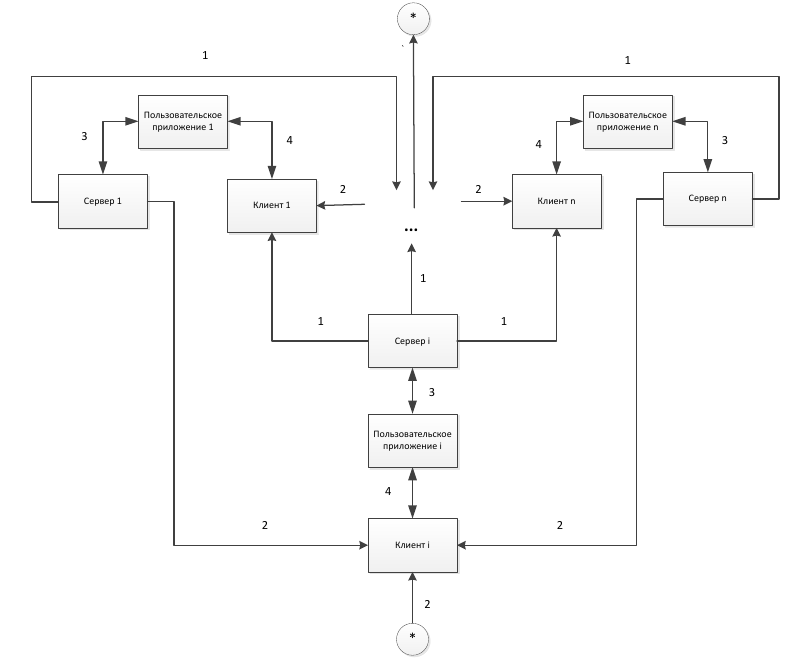
\includegraphics[scale=0.9]{pic_9}
    \caption{Схема взаимодействия между участниками сети}\label{pic_9}
\end{figure}

На рисунке \ref{pic_10}, ниже представим схему взаимодействия некоторого i-го
участника сети с другими участниками сети и покажем обмен сообщениями
между ними. Пунктирной линией по центру выделен некоторый i-й участник.
Видно как происходит запрос на передачу файла у других участников сети, а
именно у серверов, которые указаны справа. Слева и справа от i-го участника
также располагаются такие же участники, однако они показаны частично,
например, справа можно видеть лишь серверные составляющие остальных
участников сети. Также показан обмен сообщениями между клиентом и
сервером с пользовательским приложением, которое обозначено как GUI.

\begin{figure}[tb!]
    \centering
    \hspace*{-2cm}
    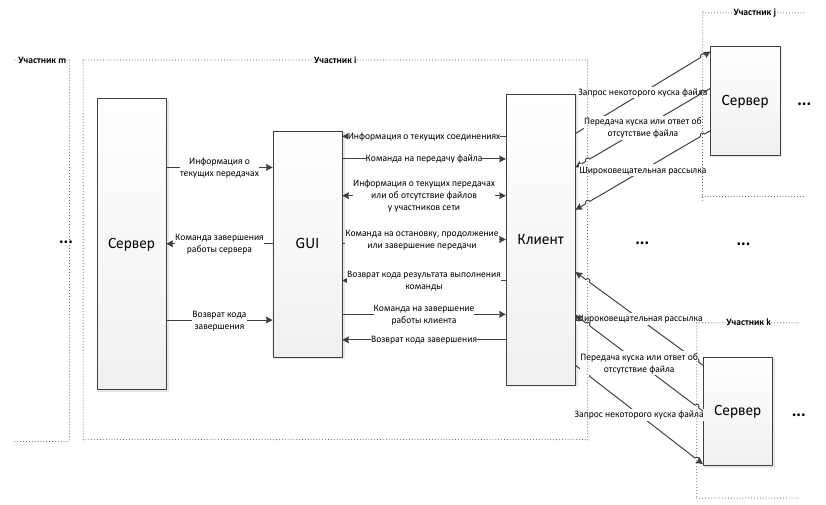
\includegraphics[scale=0.9]{pic_10}
    \caption{Схема взаимодействия между участниками и компонентами приложения}\label{pic_10}
\end{figure}

\subsection{Протокол}
Протокол разрабатывался с учетом описанных выше алгоритмов работы
клиента и сервера. Протокол представлен в виде структуры. Ниже
представим и опишем назначения полей структуры.
\begin{figure}
    \begin{lstlisting}[language=C]
struct cli_fields {
    pack_id_t pack_id;
    piece_id_t piece_id;
    perror_t error;
    file_id_t file_id;
    unsigned char hsumm[MD5_DIGEST_LENGTH];
    char file_name[FILE_NAME_MAX_LEN];
};
    \end{lstlisting}
\end{figure}
\newpar
Структура cli\_fields используется при передаче сообщения от клиента
серверу. Первое поле структуры pack\_id содержит значение номера
передаваемого пакета. Поле piece\_id равно номеру передаваемого куска. Поле
error содержит некоторое значение ошибки. Поле file\_id содержит
идентификатор файла и при передаче серверу клиентом всегда равно -1, по
данному идентификатору и номеру передаваемого куска можно однозначно
идентифицировать передачу. Далее следует поле hsumm, которое содержит
хэш-сумму передаваемого файла, оно (поле) составляет 16 байт и
генерируется стандартным алгоритмом md5. Последнее поле file\_name
содержит имя запрашиваемого файла. Необходимо заметить, что в данной
структуре отсутствует поле для данных, так как в нем нет необходимости.
Клиенту не нужно передавать данные серверу, так как он запрашивает файл.
\begin{figure}[h!]
    \begin{lstlisting}[language=C]
struct srv_fields {
    struct cli_fields cli_field;
    size_t piece_len;
    unsigned char piece[DATA_BLOCK_LEN];
};
    \end{lstlisting}
\end{figure}
\newpar
Следующая структура передается от сервера клиенту. Первое поле cli\_field
является структурой, которую клиент передает серверу, данные в этой
структуре такие же за исключением того, что поле file\_id равно некоторому
целому значению. Следующее поле piece\_len равно длине передаваемого
куска клиенту сервером. Поле piece содержит в себе кусок файла, то есть
передаваемые данные.

\subsection{Использование протокола для обмена сообщениями}
\begin{figure}[tb!]
    \centering
    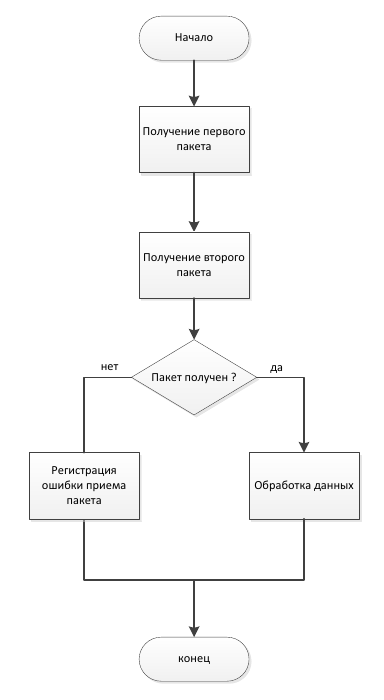
\includegraphics[scale=0.8]{pic_11}
    \caption{Блок-схема алгоритма получения пакетов}\label{pic_11}
\end{figure}
В процессе своей работы клиент и сервер обмениваются сообщениями,
которые содержат данные и информацию о том, как эти данные обрабатывать.
Протокол представлен в виде структуры, поэтому перед передачей структуру
необходимо преобразовать в последовательность байт, то есть сериализовать,
и десериализовать при получении, то есть преобразовать полученную
последовательность байтов в структуру. Однако так как размер передаваемой
последовательности (или сообщения) может быть различным (так как может
передаваться кусок файла), то необходимо преждевременно уведомить
принимающую сторону о размере передаваемого пакета (последовательности
байт). Для реализации этого передаются два пакета, первый пакет имеет
определенный размер и содержит в себе длину второго пакета. При такой
организации, принимающая сторона предварительно получает данные о
размере второго (основного) пакета. Заметим, что передачу можно
реализовать при помощи посылки одного пакета и дожидаться, когда будет
получен тот объем данных, который содержит размер всего пакета, и на
основе полученной информации продолжить ожидать получение основного
пакета, однако, был выбран первый способ, основанный на передачи двух
пакетов.
\newpar
На рисунке \ref{pic_11}, приведена схема алгоритма получения пакета.
\subsection{Мультиплексирование ввода-вывода}
Мультиплексирование ввода-вывода необходимо для того, чтобы
обрабатывать запросы, которые приходят от клиентов или серверов
участников сети. Данный механизм реализован при помощи системного
вызова select. Смысл мультиплексирования заключается в том, что процесс-
клиент или процесс-сервер блокируются на системном вызове до тех пор,
пока кто-нибудь из участников сети не пошлет некоторый запрос. После того,
как процесс-сервер или процесс-клиент получили хотя бы один запрос,
системный вызов select, на котором был заблокирован процесс-сервер или
процесс-клиент, возвращает управление. После чего анализируется
множество и делается вывод, от какого из участников пришел запрос, далее
данный запрос обрабатывается соответствующим образом. Данный механизм
ввода-вывода позволяет сэкономить на том, что нет необходимости постоянно
опрашивать всех участников на наличие пришедших запросов от них, а также
позволяет обработать случай, когда одновременно пришли два или более
запросов.
\subsection*{Выводы}
\addcontentsline{toc}{subsection}{Выводы}
Программное средство состоит из клиентской и серверной частей, а также из
пользовательского приложения. Пользовательское приложение предназначено
для предоставления доступа к основным функциям программного
обеспечения и взаимодействует с клиентской и серверной частями, которые
обеспечивают функции клиента и сервера соответственно. Под функциями
клиента понимается запрос на предоставление некоторого файла и
последующее скачивание. Под функциями сервера понимается передача
запрошенного файла, если он имеется на данном хосте. Программное
обеспечение разработано в соответствие со структурной методологией.
